\documentclass{beamer}

\mode<presentation>
{
  \usetheme{EastLansing}      
  \usecolortheme{default} 
  \usefonttheme{default}  
  \setbeamertemplate{navigation symbols}{}
  \setbeamertemplate{caption}[numbered]
} 

\usepackage[utf8]{inputenc}
\usepackage[T1]{fontenc} 
\usepackage[turkish,shorthands=:!]{babel} 
\usepackage{minted} 
\usepackage{hyperref} 

\title[Sunum]{Bilgisayar Mühendisliği Semineri Dersi Robotik Sunumu} 
\author[İ. E. G. \& A. F.]{İsmail Emir Gürbüz \inst{1} \and Asude Fışkın \inst{2}} 
\institute[Bilgisayar Müh.]{\inst{1} 20253072 \and \inst{2} 20253036} 
\date{03.05.2021} 

\begin{document}

\begin{frame}
  \titlepage
\end{frame}


\begin{frame}{Outline}
  \tableofcontents
\end{frame}

\section{Giriş}

\begin{frame}{Giriş}

\begin{itemize}
  \item Robotik nedir?
  \item Yumuşak robotik nedir? 
  \item Yumuşak robotik sistemlerin 3 boyutlu baskısı
  \item Meteryal ve metod
  \item Esnek robotların kontrol sistemleri
  \item Esnek robotların kontrol edilme şekilleri
  \item Malzeme seçimleri
  \item Bulgular
  \item Sonuç
  \item Öneriler
\end{itemize}
            
\vskip 1cm

\end{frame}

\section{ROBOTİK \LaTeX}

\subsection{Robotik Nedir?}

\begin{frame}{Robotik Nedir?}
\begin{block}{Robotik}
Robotik; robotların tasarımını, üretimini, ve kullanımı ile ilgilenen çok disiplinli bir bilim dalına verilen isimdir.
\end{block}


\begin{figure}
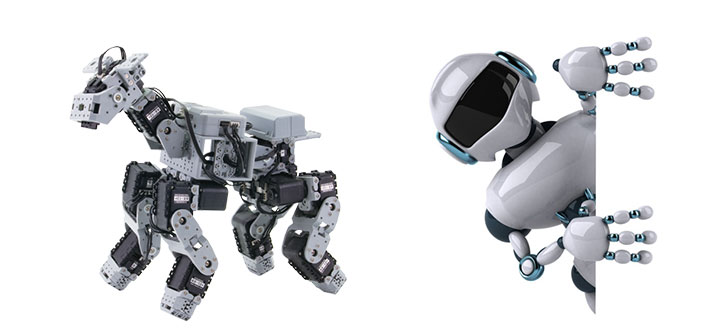
\includegraphics[width=0.5\textwidth]{robotik-01} 
\caption{\label{Şekil-1} Robotik} 
\end{figure}
\end{frame}


\subsection{Yumuşak Robotik Nedir?}
\begin{frame}{Yumuşak Robotik Nedir?}
\begin{block}{Yumuşak Robotik}
Yumuşak robotik; canlı organizmaların fiziksel özelliklerine daha çok benzeyen teknolojilere odaklanan robotiklerin alt kümelerinden biridir. Uzmanlar, yumuşak robotik yaklaşımı, robotiklerin geleneksel olarak doğrusal olan özellikleri yerine insan, hayvan ve bitki yaşamını taklit eden çok daha karmaşık modellerle değiştirdiği bir biyomimikri biçimi olarak tanımlanmaktadır.


\end{block}
\end{frame}

\begin{frame}{Yumuşak Robotik}
\begin{figure}
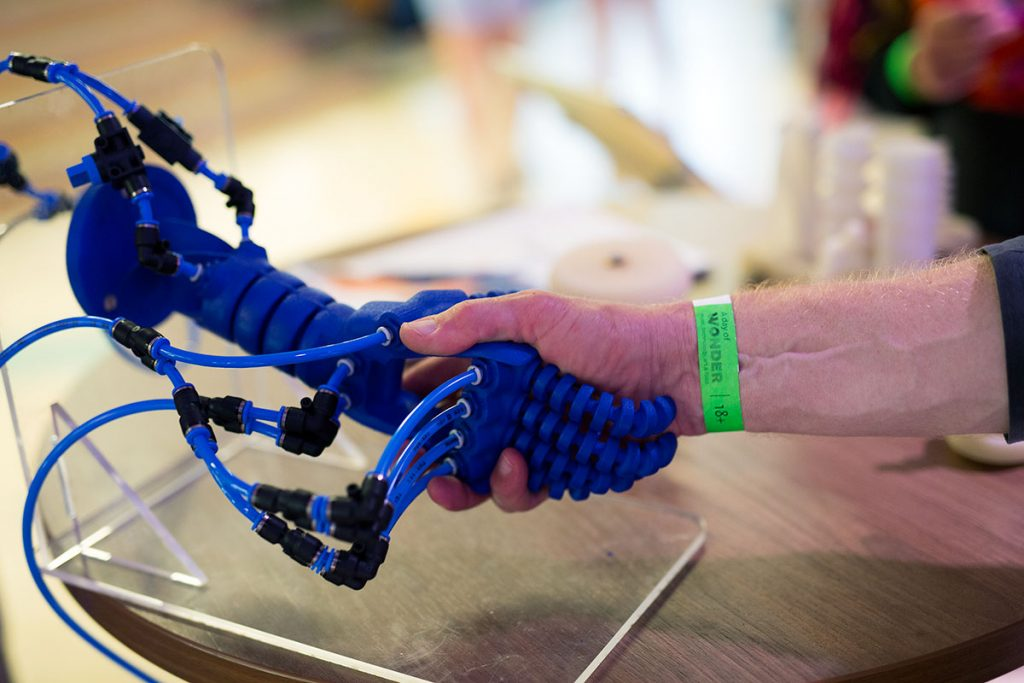
\includegraphics[width = 0.5 \textwidth]{robotik-02}
\caption{\label{Şekil-2} Yumuşak Robotik}
\end{figure}
\end{frame}
\begin{frame}{Yumuşak Robotik}
 \begin{block}
 \item Yumuşak robotiği, tanımlamanın en kolay yollarından biri geleneksel robotu tanımlamak ve kavramaktır. Robot, mevcut evriminden yıllar önce tasvir edildiği gibi, bir dizi kutu ve tüpten oluşuyordu. Yüzeyleri sert ve genellikle metaldi. Çok spesifik doğrusal yollarla hareket etme kabiliyetine sahipti. 
  \end{block}
\end{frame}

\begin{frame}{Yumuşak Robotik}
\begin{block}
\item Yumuşak robotikte ise bu durum robotların; biyolojik insanlara, hayvanlara veya bitkilere benzediği, hareket ettiği ve hissettiği yeni robotik türüne dönüştürmeyi amaçlamakta ve bu konuda güçlü çalışmalar yapmaktadır. 
\end{block}
\begin{figure}
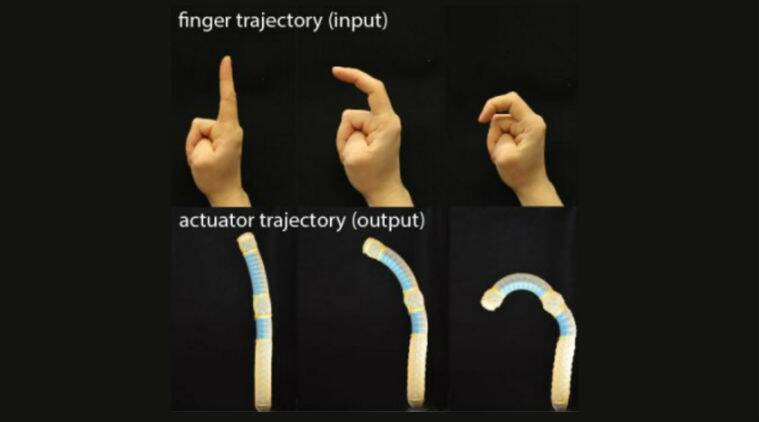
\includegraphics[width = 0.5 \textwidth]{robotik-03}
\caption{\label{Şekil-3} Yumuşak Robotik}
\end{figure}
\end{frame}

\begin{frame}{Yumuşak Robotik}
\begin{block}
\item Yumuşak robotiğin temel özelliklerinden biri, sert bir metal yüzey yerine, insan derisi gibi hareket edebilen küçük metal parçalardan oluşan, çok yönlü bir şekilde hareket etme kabiliyetine sahip, karmaşık, çok bölümlü birimlerden oluşturulmasıdır.
\end{block}

\begin{figure}
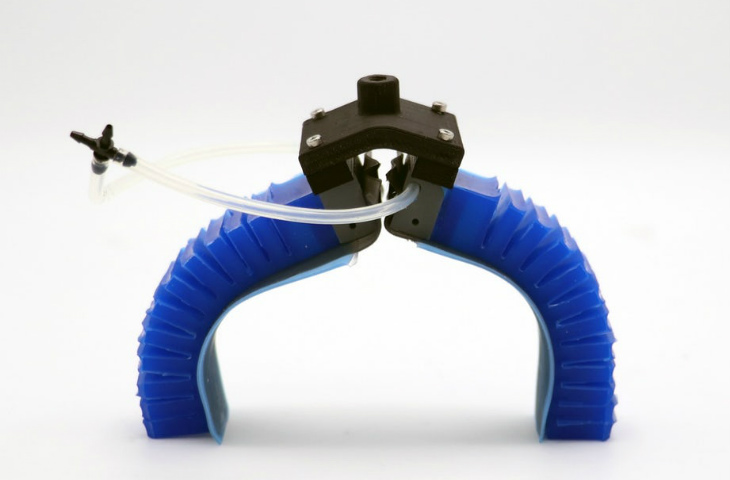
\includegraphics[width = 0.5 \textwidth]{robotik-04}
\caption{\label{Şekil-4} Yumuşak Robotik}
\end{figure}

\end{frame}

\subsection{Yumuşak Robotik Sistemlerin 3 Boyutlu Baskısı}

\begin{frame}{Yumuşak Robotik Sistemlerin 3 Boyutlu Baskısı}
\begin{block}
\item Yumuşak malzemelerdeki ve eklemeli üretim teknolojilerindeki gelişmeler, atlama, karmaşık 3B hareketler, kavrama ve bırakma gibi sofistike yeteneklere sahip yumuşak robotların tasarımını mümkün kılmıştır.

\end{block}

\begin{figure}
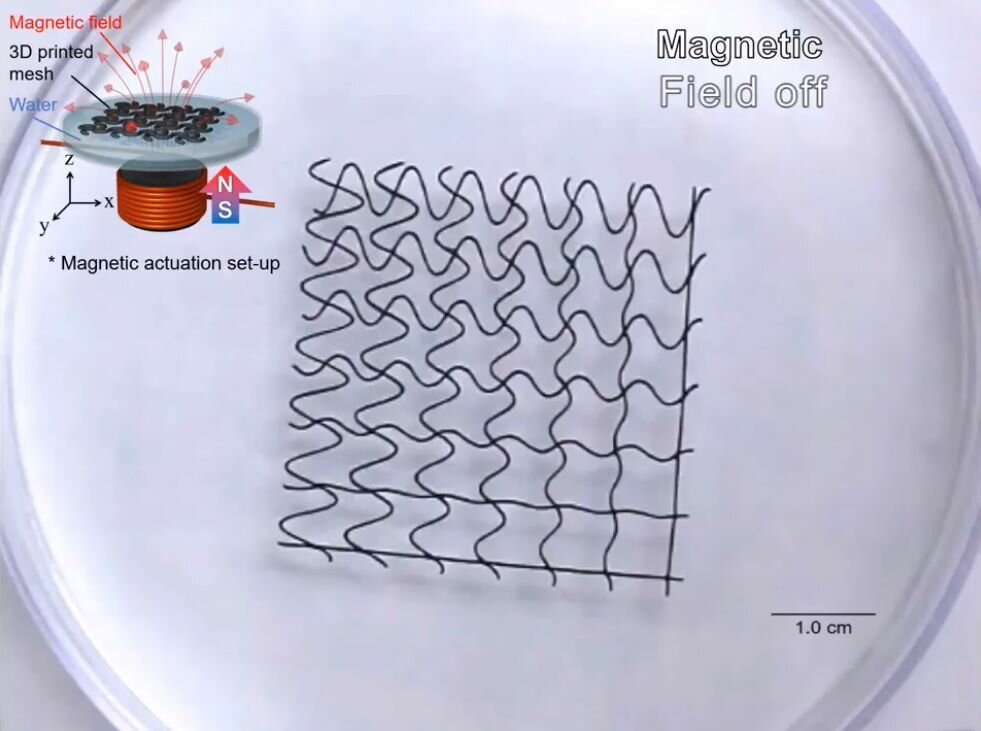
\includegraphics[width = 0.5 \textwidth]{robotik-05}
\caption{\label{Şekil-5} Yumuşak Robotik}
\end{figure}

\end{frame}

\begin{frame}{Meteryal ve Metod}
\begin{block}
\item Esnek robotlar, esnek olarak hareketliliğini gerçekleştirebilmesi için yumuşak malzeme özelliklerinden, özellikle de elastiklikten yararlanmaktır. Elastiklik özelliği nedeniyle, robotların gövdesinin ve işlevlerinin çalışma ortamlarına uygun olmasını sağlayan kontrolün dikkate alınması gerekir. Bu kontrolü sağlıya bilmek için, robotlara uygun kontrol sistemlerin seçilmesi gerekmektedir.
\item Ayrıca esnek robotların ayırt edici en önemli özelliklerinden biride robotların yapımında kullanılan gövdeye uygun şekilde güç aktarımını sağlayan güç kaynaklarının seçilmesidir.
\end{block}
\end{frame}

\subsection{Meteryal ve Metod}

\begin{frame}{Meteryal ve Metod}
\begin{block}
\item Bu bölümde bir esnek robotun üretimi sırasında gerçekleştirilen kontrol sistemleri, kontrol edilme şekilleri ve malzeme seçimlerini inceleyeceğiz.
\end{block}
\begin{figure}
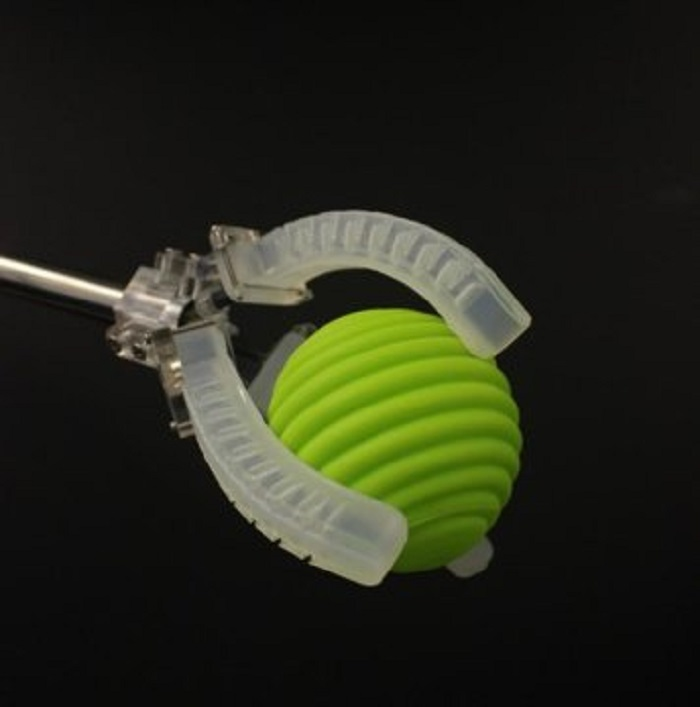
\includegraphics[width = 1 \textwidth]{robotik-06}
\caption{\label{Şekil-6} Esnek Robotik}
\end{figure}

\end{frame}

\subsection{Esnek Robotların Kontrol Sistemleri}

\begin{frame}{Esnek Robotların Kontrol Sistemleri}
\begin{block}
\item Robotların kontrol sistemleri geri beslemeli ve geri beslemesiz olmak üzere iki temel sınıfa ayrılabilirler. 

\item Kontrol edilecek sistemde algılayıcılar bulunuyorsa ve bu algılayıcılardan gelen bilgi kontrol sistemine girdi olarak uygulanıyorsa bu tip sistemlere \textbf{geri beslemeli sistem} denir .

\item \textbf{Geri beslemesiz kontrol sistemi}nde ise kontrol sistem ile kontrollü değişken arasında doğrudan bir bağlantı bulunmamaktadır. 

\item Esnek robotların kontrol yöntemlerine bakıldığında son yıllardaki çalışmalarda geri beslemeli \textbf{Oransal kontrol, Oransal-Türevsel, Oransal-Türevsel-İntegral kontrol ve Kayma Kipli} kontrolyapıları kullanılmıştır.
\end{block}
\end{frame}

\begin{frame}
\begin{block}{Oransal (p) Kontrol}
\item Oransal kontrol en çok kullanılan doğrusal geri beslemeli kontrol sistemlerinden bir tanesidir. Orasal kontrol yardımıyla esnek robotlarda akışkanların kontrolü sağlanmıştır. 

\item Oransal kontrolcü, çıkışına hatanın belirli bir “kazanç” değeri ile çarpımı kadar etki göstermektedir . Amacı ise sabit durum hatasını azaltmaktır. Kazanç değeri artıkça kararlı durum hatası azalmaktadır.
\end{block}
\end{frame}

\begin{frame}
\begin{block}{Oransal-Türevsel (pd) Kontrol}
\item PD kontrolörünün kullanılmasının amacı, sistem müdahalesinin gelecekteki hatasını tahmin etme yeteneğine sahip olduğundan, kontrolü iyileştirerek sistemin stabilitesini arttırmaktır. 

\item D modu, hata çıkışındaki ani değişikliklerden kaynaklanan kontrol çıktısında meydana gelen ani değişikliklerin önlenmesi için çıkış değişkeninin değişimi ile orantılı olacak şekilde tasarlanmıştır
\end{block}
\end{frame}

\begin{frame}
\begin{block}{Oransal-Türevsel-İntegral (pıd) Kontrol}
\item PID kontrol ünitesi, kararlı durum hatası sıfır, hızlı tepki (kısa yükselme süresi), salınım ve daha yüksek kararlılık dahil olmak üzere optimum kontrol dinamiğine sahiptir.

\item PI kontrolörüne ek olarak bir türev kazanç bileşeninin kullanılmasının gerekliliği, sistemin çıkış yanıtında meydana gelen aşma ve salınımların ortadan kaldırılması içindir
\end{block}
\end{frame}

\begin{frame}
\begin{block}{Kayma Kipli (kkk) Kontrol}
\item Doğrusal olmayan veya değişen parametrelere sahip sistemlerin kontrolü için kullanılan en iyi kontrol yöntemlerinden birisi de Kayma Kipli Kontroldür. Modellenmemiş dinamikler ve bozucu girişlerin etkili olduğu durumlarda bu yöntem dayanıklı birkontrol yöntemi sağlar. 

\item KKK yönteminin asıl amacı sistem kaçıncı dereceden olursa olsun sistemin davranışını birinci dereceye
indirgeyerek kontrol girişini belirlemek ve sistemin birinci derece gibi davranmasını sağlamaktır. Böylece, bu kontrol yöntemi sayesinde modellenmemiş parametrelerin ve bozucu girişlerin etkisinin görüldüğü durumlarda bile kararlı bir kontrol elde edilmiş olur.
\end{block}
\end{frame}

\subsection{Esnek Robotların Kontrol Edilme Şekilleri}

\begin{frame}{Esnek Robotların Kontrol Edilme Şekilleri}
\begin{block}
\item Esnek robotların hareketleri katı cisimlerin kontrolünden farklı olarak altı serbestlik derecesiyle tanımlanabilmektedir(x, y ve z ekseni etrafında üç dönüş ve üç çeviri). Esnek malzemeler elastik, büküleme, kırılma ve gerilme vb. yapılara sahiptir.

\item Esnek bir robotun gövdesinin hareket ettirilebilmesi için çeşitli yöntemler bulunmaktadır. Esnek robotların ayırt edici en önemli özellikleri robotların yapımında kullanılan aktüatörler ve gövdeye uygun şekilde güç aktarımını sağlayan güç kaynaklarıdır.
\end{block}
\end{frame}

\begin{frame}
\begin{block}
\item Güç aktarım şekillerine bakıldığında 4 ana grupta incelenmiştir. Bunlar: \textbf{Hidrolik sistemler, pnömatik sistemler, elektriksel sistemler ve kimyasal sistemler}dir.
\end{block}
\end{frame}

\begin{frame}
\begin{block}{Hidrolik Sistemler}
Günümüzde “hidrolik” sıvı akışkanlar aracılığıyla kuvvetlerin ve hareketlerin iletilmesini sağlayan sistemlerdir. Elektrik motorunun tahrik ettiği hidrolik pompa ile akışkanın belirli bir basınçta ve debide basılmasını sağlar. Bu hidrolik enerji ile doğrusal, dairesel ve açısal hareketin üretilmesine neden olur. Esnek robotlar ile yapılan çalışmalar incelendiğinde güç aktarımları hidrolik sistemler ile sağlanmış olanlar olduğu da görülmüştür. Daha çok akışkan olarak yaşam kaynağımız olan su ile yapıldıkları göze çarpmaktadır.
\end{block}
\begin{figure}
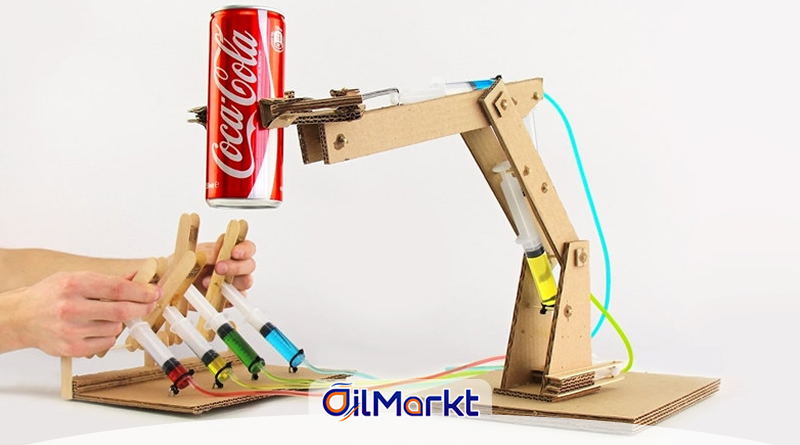
\includegraphics[width = 0.5 \textwidth]{robotik-07}
\caption{\label{Şekil-7} Esnek Robotik}
\end{figure}
\end{frame}

\begin{frame}
\begin{block}{Pnömatik Sistemler}
Sıkıştırılmış hava ile çalışan sistemlere pnomatik sistemler denir. Genellikle ortamda bulunan havayı alarak mekanik enerjiye çeviren sistemlerdir. Pnomatik enerjiyi kullanarak enerjinin açısal, dairesel ve doğrusal bir şekilde hareket etmesini sağlamaktadırlar. Pnomatik sistemler için kullanılacak olan hava basıncı genellikle kompresör yardımı ile elde edilmektedir. 
\end{block}

\begin{figure}
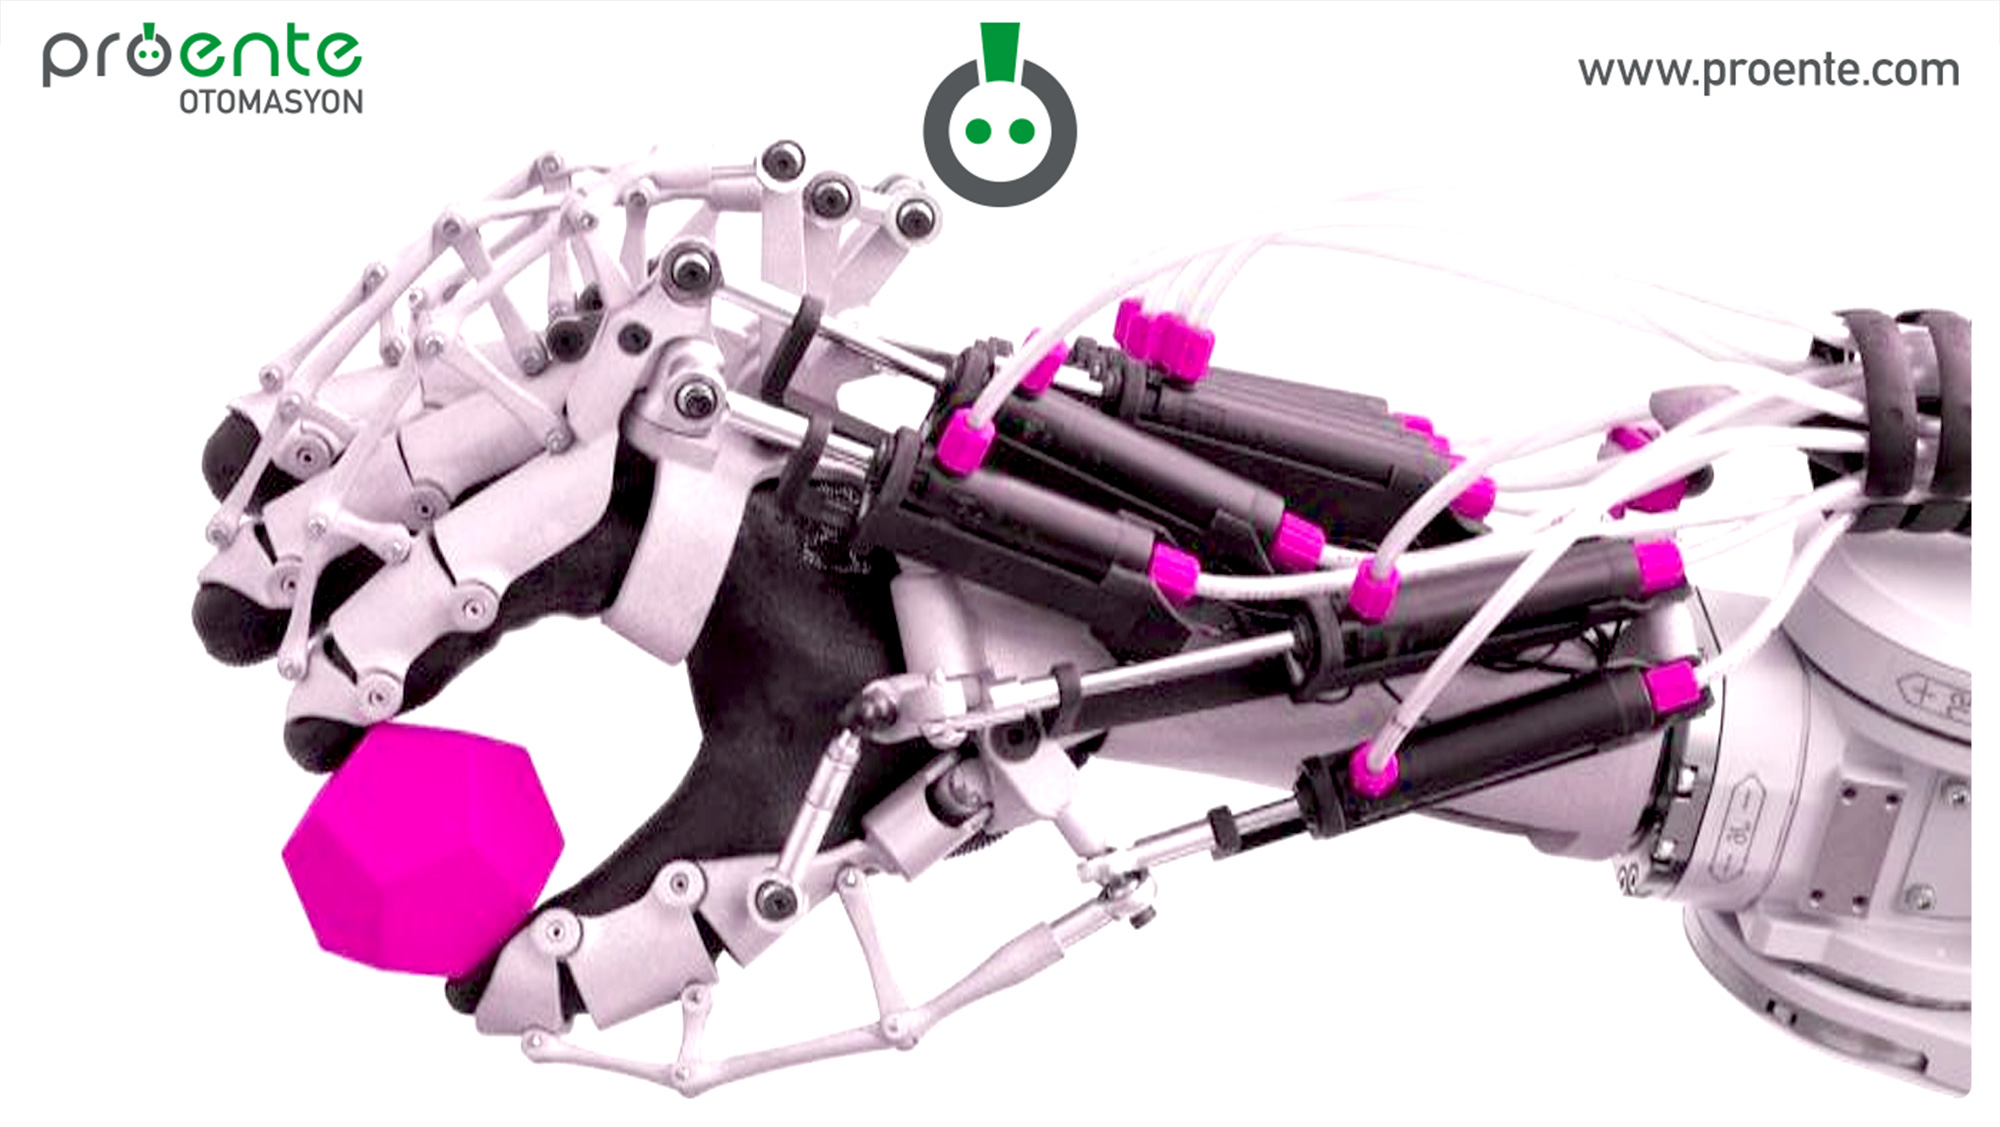
\includegraphics[width = 0.5 \textwidth]{robotik-08}
\caption{\label{Şekil-8} Esnek Robotik}
\end{figure}
\end{frame}

\begin{frame}
\begin{block}{Pnömatik Sistemler}
Esnek robotların bir zorluğu ise robotu harekete geçirmek için taşınabilir bir güç kaynağı bulabilmektir. Pnömatik sistemler için mevcut akışkanın güç kaynakları esnek değildir ve genellikle büyük ve hantaldır. Basınçları sağlamak için kompresörler veya pompalar ve sıkıştırılmış hava silindirleri kullanılır. Minyatür kompresörler, elektrik enerjisini verimsiz kullanırlar ve silindirler uzun ömürlü olmazlar. Kimyasal olarak çalıştırılan portatif basınç kaynağı bir hidrojen peroksit monopropellant kullanılarak basınçlı gaz üretir.
\end{block}
\end{frame}

\begin{frame}
\begin{block}{Pnömatik Sistemler}
Pnömatik sistemler de, elektrik kontrolörleri gibi esnek ve hafif elektrik güç kaynakları gerektirirler. Bundan dolayı grafen, organik polimer, gömülü iletken kumaş bazlı bataryalar kullanılmaktadır
\end{block}

\begin{figure}
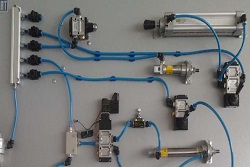
\includegraphics[width = 0.5 \textwidth]{robotik-18}
\caption{\label{Şekil-9} Esnek Robotik}
\end{figure}
\end{frame}

\begin{frame}
\begin{block}{Elektriksel Sistemler}
Genellikle elektriği kullanarak mekanik enerjiye çeviren sistemlerdir. Elektrik enerjisini alarak enerjiyi açısal, dairesel ve doğrusal bir şekilde hareket ettirmeyi sağlamaktadırlar. Rijit robot teknolojisinde en çok kullanılan kontrol edilme şekillerinden biridir. Bu teknolojide en çok kullanılan servo motorlar ve fırçasız DC motorlar bunlara örnek verilebilir.
\end{block}

\begin{figure}
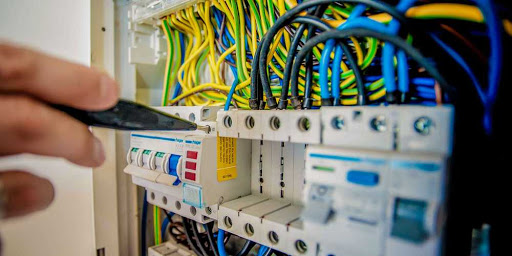
\includegraphics[width = 0.5 \textwidth]{robotik-09}
\caption{\label{Şekil-10} Esnek Robotik}
\end{figure}
\end{frame}

\begin{frame}
\begin{block}{Kimyasal Sistemler}
\item Son dönemlerde yeni bir araştırma alanı olan kimyasal tepkiler robotik alanında gerçekleştirilen çalışmalara hızla girmiştir.
\item Kimyasal enerji moleküldeki atomların tepkimesi sonucu açığa çıkan enerjidir. Kimyasal enerjinin mekanik enerjiye dönüşmesi esnek robotlarda yapılan çalışmalarda kullanılmaya başlanmıştır 
\end{block}
\begin{figure}
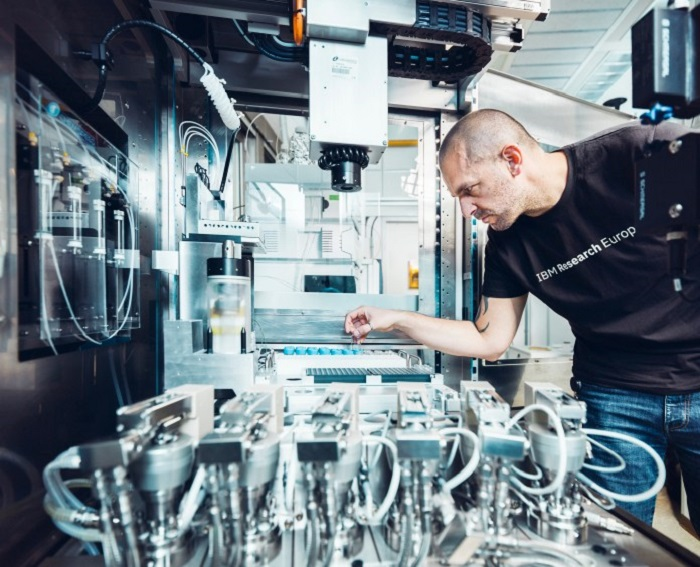
\includegraphics[width = 0,5 \textwidth]{robotik-10}
\caption{\label{Şekil-11} Esnek Robotik}
\end{figure}
\end{frame}

\subsection{Malzeme Seçimi}

\begin{frame}{Malzeme Seçimi}
\begin{block}
\item Son yıllarda dünya çapında birçok malzeme ile birçok farklı çalışma alanları ile karşılaşılmaktadır. Esnek robot ile yapılan çalışmalara bakıldığında aktüatör olarak daha çok fiber takviyeli aktüatörlerin kullanıldığı
görülmektedir. Fiber takviyeli aktüatörlerin temel tasarımına bakıldığında uzayabilir olmayan takviyeler ile sarılmış bir elastomer iç lastikten oluşmaktadır. Çekme kuvveti altında çok yüksek oranda uzayabilen, kuvvet kaldırıldığında ise başlangıç uzunluğuna geri dönebilen çapraz bağlanmış kauçuğumsu polimerlere 
\textbf{elastomer malzemeler} denir.
\end{block}
\end{frame}

\begin{frame}
\begin{block}
\item Fiber takviyeli aktüatörün iç lastiği bir balon gibi davranır; hava her yöne doğru genişlemeye başlar. İç lastik, uzamayan takviyeler ile sarıldığında radyal olarak genişlemesi engellenir ve hava verildiğinde sadece eksenel yönde ilerlemesi sağlanır.
Fiber takviyeli aktüatöre uzamayan bir malzeme tabakası eklenirse aktüatörün o tabaka bölgesinde genişlemesi engellenir. Diğer tabaka genişlemeye devam ettirilirse uzamayan tabaka etrafında bükülme hareketi sağlanmış olur.
\end{block}
\begin{figure}
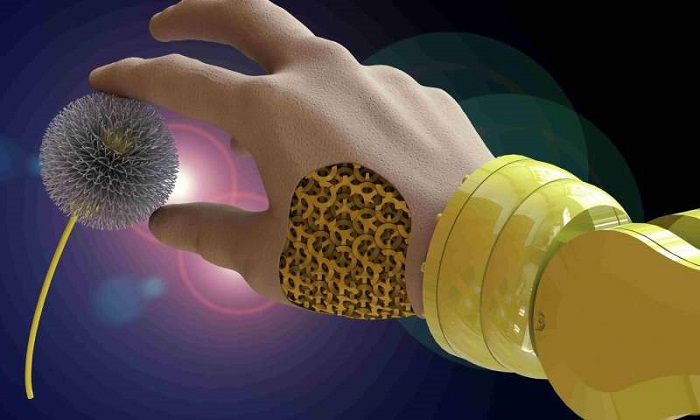
\includegraphics[width = 0.5 \textwidth]{robotik-11}
\caption{\label{Şekil-12} Malzeme Seçimi}
\end{figure}
\end{frame}

\begin{frame}
\begin{block}{Fiber takviyeli aktüatör tasarlanırken;}
\item İçi boş yarım silindir şeklinde elastomer malzemeden oluşan iç lastik bölgesinin kalıbı oluşturulur.
\item Hava verildiğinde gerilmeyi azaltan fiberglas malzemeden oluşan gerilme sınırlayıcı tabaka yerleştirilir.
\item Radyal gerilmeleri sınırlayarak uzamayı sağlayan Kevlar ipliği ile sarımı yapılan takviyeler gerçekleştirilir.
\item  Son olarak ise Kevlar ipliğinin sabitlenmesi için dış deri tabakası oluşturulur.
\item Aktüatörün iç lastik bölgesini oluşturulurken kullanılacak malzemeler Wacker Chemie AG firması tarafından üretilen Elastosil M4601 silikon veya Smooth-On Inc. firması tarafından üretilen Dragon Skin 30 dur. Takviyeleri yerinde tutmak için uygulanan dış deri tabakası için Ecoflex 20 veya Dragon Skin 20 gibi daha düşük sertlikteki malzemeler kullanılır.
\end{block}
\end{frame}

\subsection{BULGULAR}

\begin{frame}{Bulgular}
\begin{block}
\item Esnek robotlar ile ilgili literatür çalışmaları incelendiğinde en önemli kriterlerin tasarımda kullanılan donanım elemanları ve esnek malzemelerinin seçimi olduğu sonucuna varılmıştır. Esnek robotlar, seçilen malzemeler ile tasarlanırken daha çok kalıp oluşturularak modellenme gerçekleştirilir. Bu kalıplar 3 boyutlu yazıcılar tarafından imal edilmiştir
\end{block}
\end{frame}

\begin{frame}
\begin{figure}[ht]
\centering
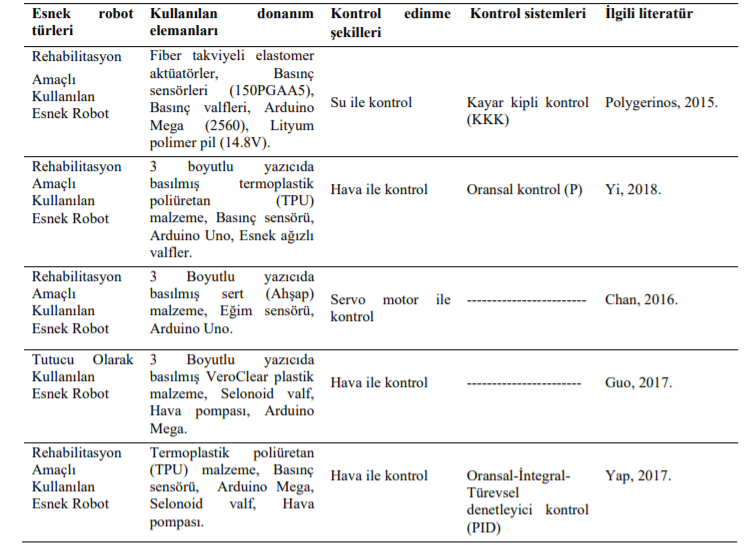
\includegraphics[bb=0 0 220 80]{robotik-12}
\caption{\label{Tablo-1}}
\end{figure}
\begin{figure}
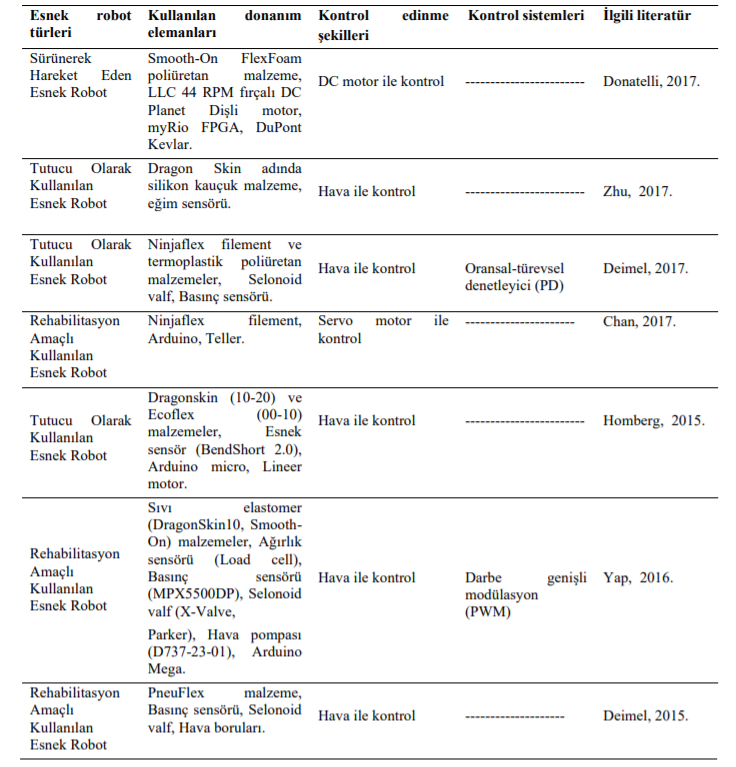
\includegraphics[width = 0.5 \textwidth]{robotik-13}
\caption{\label{Tablo-1}}
\end{figure}
\end{frame}

\begin{frame}
\begin{block}
 \item Tablo 1’de verildiği üzere incelenen makalelerin hangi tür esnek robot olduğu ve onlara ait kullanılan donanım elemanları, kontrol edilme şekilleri ve kontrol sistemleri belirtilmiştir. Ayrıca hava ve su ile kontrol edilen çalışmalarda basınçlı hava üretmek için kompresörler kullanılmıştır. Oluşturulan havanın istenilen basınçta sisteme verilmesi için basınç sensörleri ile ölçüm yapılmıştır. 
 
 \item Gerekli olan basınçlı havayı yönlendirmek için daha çok selonoid valfler tercih edilmiştir
 
 \item Selonid valfleri, basınç sensörlerini, motorları ve kompresörleri kontrol etmek için ise Arduino, FPGA gibi farklı tip kontrol kartları tercih edilmiştir. Ayrıca esnek robotlarda güç aktarım şekli elektrik olan motorlar da kullanılabilinir. Motorlar ile yapılan esnek robot çalışmalarında daha çok servo motor ve fırçalı DC motor kullanılmıştır.
\end{block}
\end{frame}

\subsection{SONUÇ }

\begin{frame}{SONUÇ}
\begin{block}
\item Yaptığımız araştırmalar sonucunda esnek robotların kullanım alanları sürünerek hareket edebilen, yüzebilen, rehabilitasyon amaçlı ve tutucular olarak gruplandırılmıştır. 

\item Sürünerek hareket edebilen esnek robotlar yuvarlak, yassı, halkalı solucanlar ve tırtıl gibi omurgasız hayvanların yanı sıra yılan gibi omurgalı hayvanların hareketlerinden esinlenilerek gerçekleştirildiği görülmüştür.
\end{block}
\begin{figure}
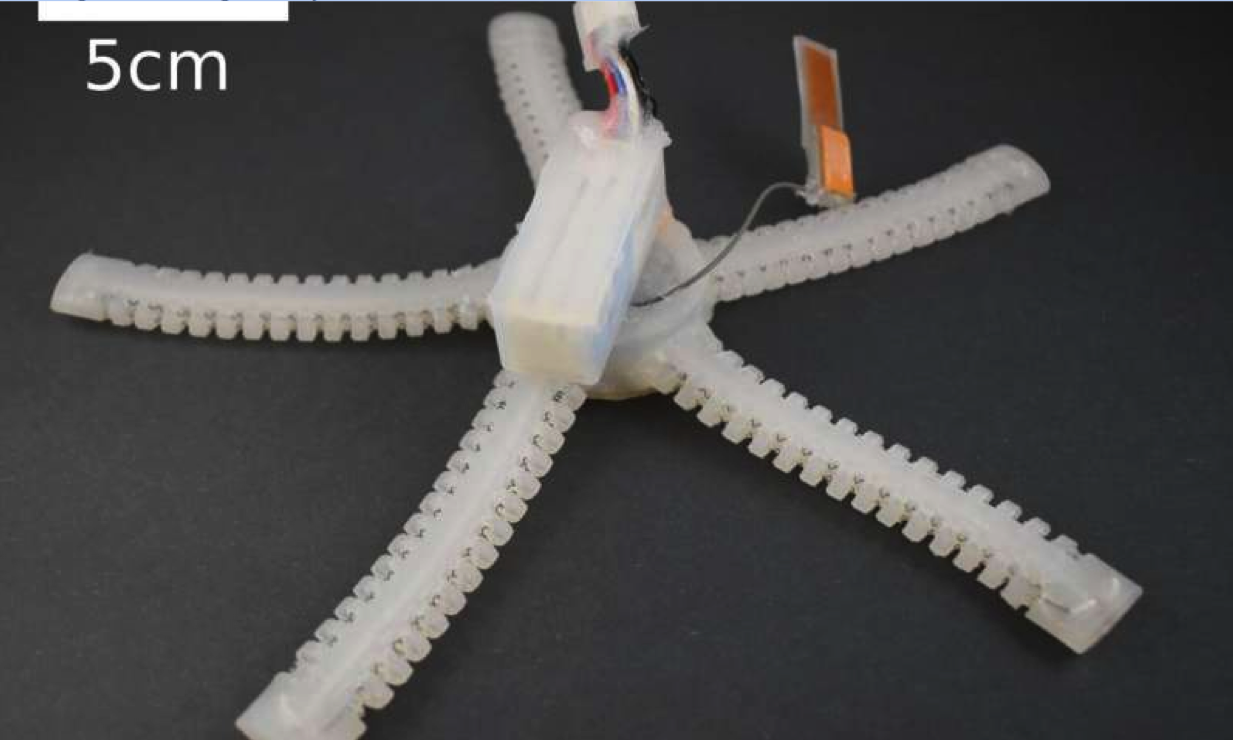
\includegraphics[width = 0.5 \textwidth]{robotik-14}
\caption{\label{Şekil-13} Esnek Robot}
\end{figure}
\end{frame}

\begin{frame}{SONUÇ}
\begin{block}
\item Yüzerek hareket eden esnek robotlar da daha çok balıklar ve kafadanbacaklılar grubuna giren ahtapot dan yararlanılmıştır.

\begin{figure}
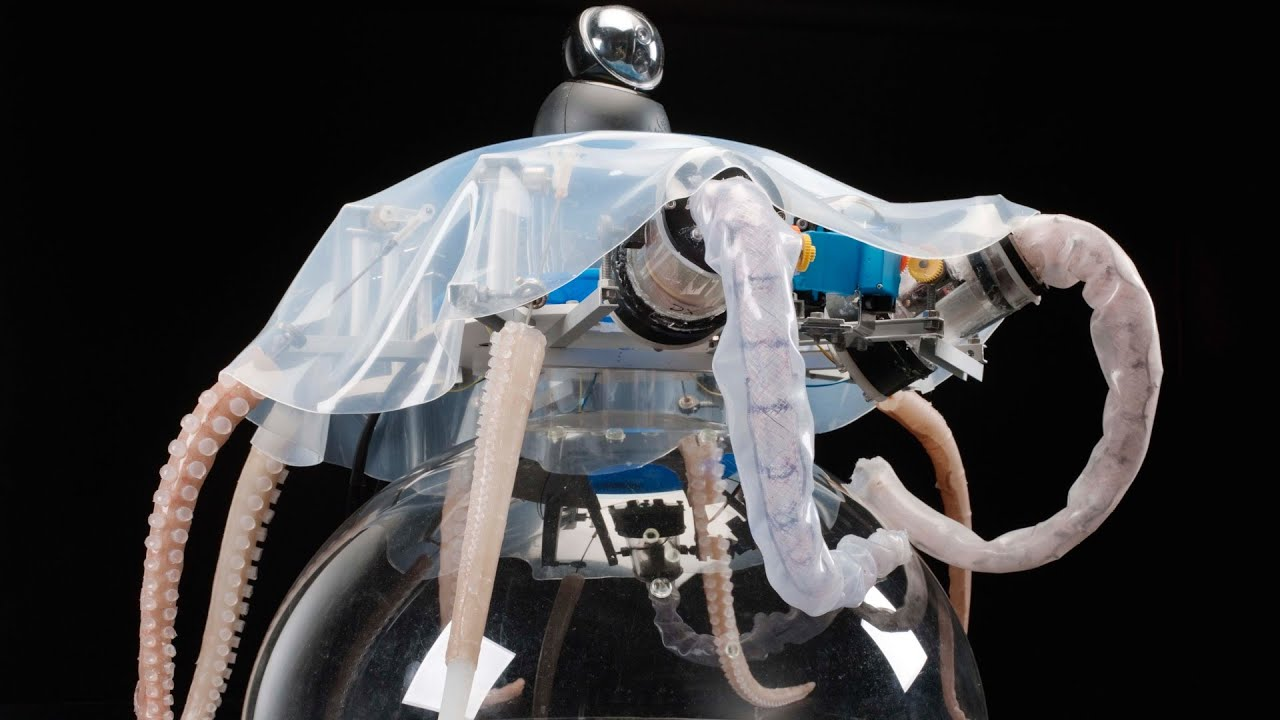
\includegraphics[width = 0.5 \textwidth]{robotik-15}
\caption{\label{Şekil-14} Esnek Robotik}
\end{figure}
\end{block}
\end{frame}

\begin{frame}{SONUÇ}
\begin{block}
\item Rehabilitasyon amaçlı esnek robotlar daha çok fonksiyonel kavrama hastalığı olan bireyler için el rehabilitasyonunu güçlendirmek üzere insanların el ve bilek hareketleri ilham alınmıştır. 

\item Esnek tutucularda ise insanların el ve bilek hareketlerinin yanı sıra gecko gibi
sürüngenlerin yapışkanlığından da yararlanılmıştır. 
\begin{figure}
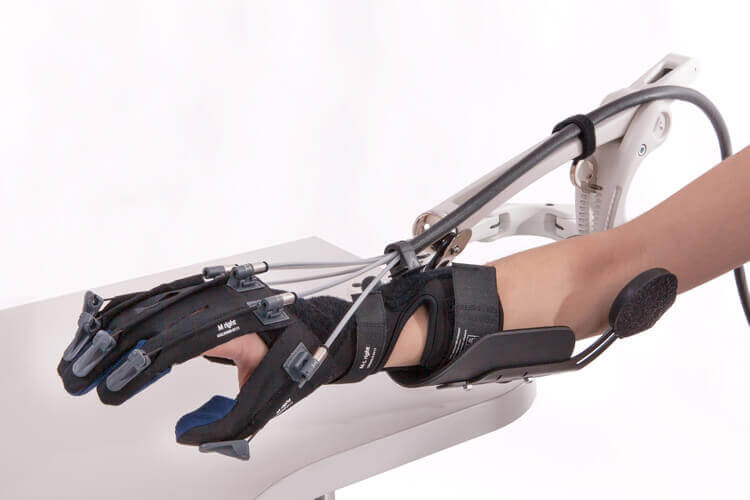
\includegraphics[width = 0.5 \textwidth]{robotik-16}
\caption{\label{Şekil-15} Esnek Robotik}
\end{figure}
\end{block}
\end{frame}

\begin{frame}{SONUÇ}
\begin{block}
\item Esnek robotlar ile yapılan çalışmalar incelendiğinde güç aktarımlarının daha çok hidrolik (Su), pnömatik (Hava), kimyasal ve elektrik (Motor) ile sağlandığı görülmüştür Esnek robotların hareketliliğini sağlayan aktüatörlerin iç lastik bölgesinde daha çok Elastosil M4601 silikon veya Dragon Skin 30 malzemelerinden biri kullanıldığı görülmüştür. Aktuatörün dış deri tabakası için ise daha düşük sertlikteki malzemelerden olan Ecoflex 20 veya Dragon Skin 20 kullanılmıştır.
\end{block}
\end{frame}

\begin{frame}
\begin{block}
\item Esnek robotlar tasarlanırken öncelikle esnek malzemenin dökümü için bir kalıp hazırlandığı görülmüştür. Bu kalıplar 3 boyutlu yazıcılar tarafından üretilmiştir. Kalıpları oluşturulan tasarımlara Smooth-On FlexFoam poliüretan, Termoplastik poliüretan,Dragonskin (10-20) ve Ecoflex (00-10) silikon malzemeleri gibi farklı çeşit esnek malzemeler dökülmüştür. 

\item Daha sonra hava ile kontrol edinme şekillerinde vakum pompası veya kompresör, sayesinde robotun kanallarına hava verilerek robotların hareketi sağlanmıştır
\end{block}
\end{frame}

\begin{frame}
\begin{block}
\item Basınç sensörleri, kanallara verilecek olan basınçları ayarlamıştır. Robotların istenilen hareketi sağlaması için uygun kanallara hava akışını yönlendiren selonid valfler kullanılmıştır. Esnek robotların kullanıcının istediğini kontrollü bir şekilde yapabilmesi için bütün devre elemanlarını kontrol eden Arduino, FPGA gibi farklı tip kontrol kartları tercih edilmiştir.

\item Ayrıca hidrolik sistemli esnek robotların hareketinin sağlanması için gerekli akışkanı depolayan bir tank ve bu tanktan akışkanı kanallara gönderen bir pompa kullanılmıştır. Akışkan valfleri sayesinde akışkanların yönlendirilmesi sağlanmıştır.
\end{block}
\end{frame}

\begin{frame}
\begin{block}
\item Esnek robotlar sayesinde insanların işleri daha da kolaylaşmıştır. Bunun nedeni ise esnek robotların diğer robotlara göre daha esnek bir şekilde hareketliliğinin sağlanması ve geliştirilen yöntemler sayesinde sarsıntılar azalmasına neden olmuştur. \cite{Wallin}

\item Ayrıca güvensiz ortamlarda ve tekrarlı işlerde esnek robotlar çokça kullanılmaya başlanmıştır.\cite{Yetkin}
\end{block}
\begin{figure}
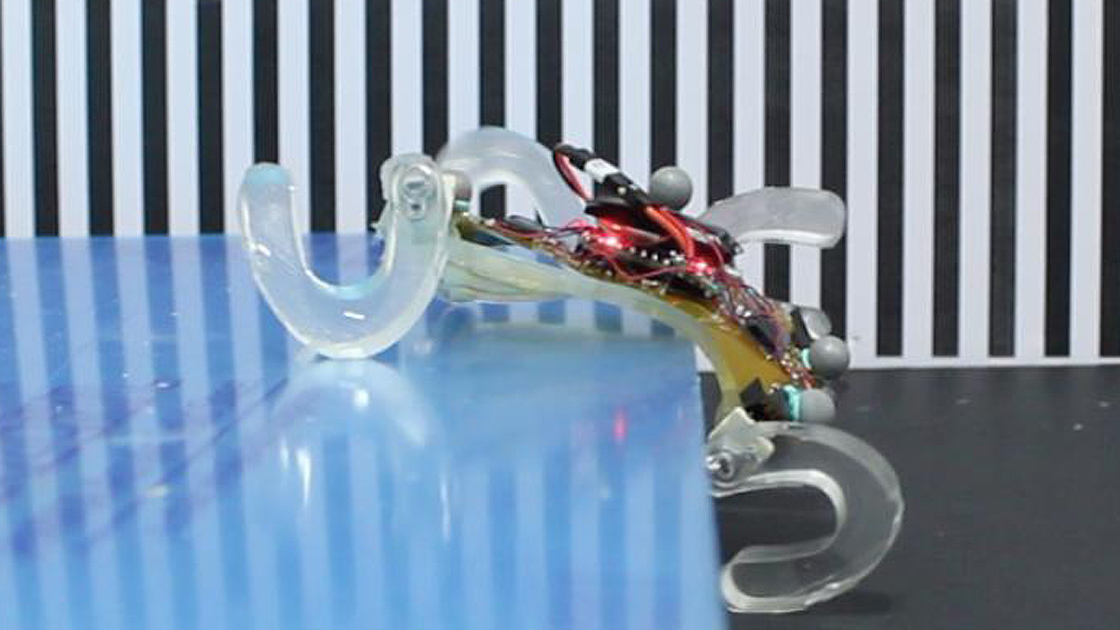
\includegraphics[width = 0.5 \textwidth]{robotik-17}
\caption{\label{Şekil-16}}
\end{figure}
\end{frame}

\subsection{ÖNERİLER }

\begin{frame}{ÖNERİLER}
%\begin{block}
%\end{block}
\item İleriki çalışmalarda rehabilitasyon amaçlı kullanılan esnek bir el tasarlanarak bütün parmakların hava ile kontrolü sağlanacaktır.

\item Yapılmış olan esnek robotların ANSYS paket programında zamana bağlı akış analizi yapılabilir. Daha farklı malzemelerin karışımı ile olan yeni bir kimyasal madde kullanılarak esnek parmaklar yapılabilir. 

\item Yapılmış olan esnek parmak farklı kontrol yöntemleri ile kontrol edilebilir.
%\end{block}
\end{frame}


\subsection{KAYNAKÇA}
\begin{frame}[allowframebreaks]{Kaynaklar}
\bibliographystyle{plain}
\scriptsize
\bibliography{kaynaklar}
\end{frame}

\end{document}